\documentclass{standalone}
%
\usepackage{tikz}
\usetikzlibrary{backgrounds,arrows.meta,shapes.callouts}
\usepackage{xcolor}
%
\definecolor{space}{HTML}{1F2C4E}
\definecolor{earth}{HTML}{0089FA}
\definecolor{dida}{HTML}{FFDE00}
\definecolor{title}{HTML}{FBA706}
\definecolor{galaxy}{HTML}{4278A4}
\definecolor{paper01}{HTML}{BE8A3F}
\definecolor{paper02}{HTML}{E5D09B}
%
\usepackage{fontspec}
\setmainfont{Open Dyslexic}
%
\title{Vite d'astronome}
\begin{document}
	\begin{tikzpicture}[background rectangle/.style={fill=white},show background rectangle,>={[inset=0,angle'=27]Stealth}]
		% title
		\draw [black,ultra thick,fill=title] (0,12.8) rectangle (30,16.8);
		\node at (15,14.8) {\textcolor{black}{\fontsize{75}{76}\selectfont Vite d'astronome}};
		% stripe
		\begin{scope}[shift={(0,12)}]
			\draw [fill=earth!50!white, thick] (14.5,0) rectangle (26.5,-115);
			\foreach \i in {0,1,...,11}
			{
				\draw [fill=white, thick] (14.75+\i,-0.5) rectangle (15.25+\i,-1);
			}
			%
			\foreach \j in {0,1,...,11}
			{
				\draw [fill=white, thick] (14.75+\j,-112.5) rectangle (15.25+\j,-113);
			}
		\end{scope}
		%
		% Caroline Herschel
		%
		\begin{scope}[shift={(0,8)}]
			\draw [fill=earth!50!space, thick] (3,0.9) rectangle (13,-10.9);
			\node at (8,-5) {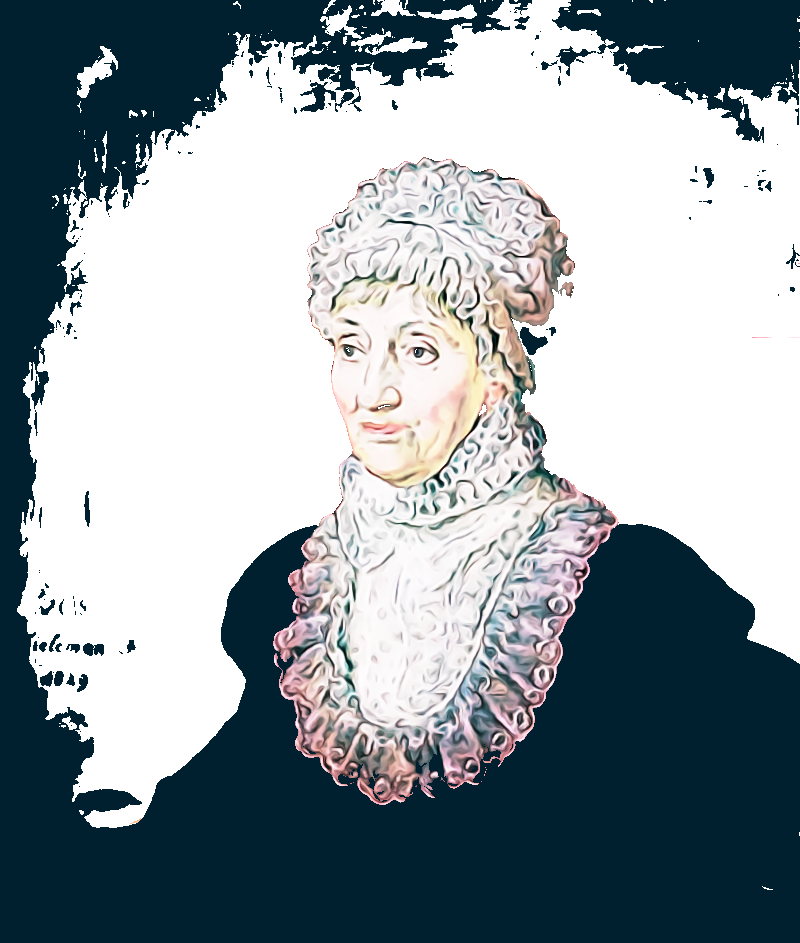
\includegraphics[width=10cm]{caroline_herschel}};
			%
			\draw [fill=galaxy, thick] (4.8,-10.5) rectangle (11.2,-11.5);
			\node at (8,-11) {\textcolor{black}{\fontsize{18}{19}\selectfont Caroline Herschel}};
			%
			\draw [fill=title, thick] (14,0.9) rectangle (27,1.8);
			\node (example-textwidth-2) [right, align=left, text width=12cm, color=black, font=\fontsize{18pt}{19pt}\selectfont] at (15,1.3) {\textbf{16 marzo 1750}};
			%
			\node (example-textwidth-2) [right, align=left, text width=12cm, color=black, font=\fontsize{18pt}{19pt}\selectfont] at (15,-0.1) {Sorella di \textbf{William Herschel}};
			%
			\shade [bottom color=paper02,top color=paper01]	(14,-1.1) rectangle (27,-6.3);
			\draw [thick] (14,-1.1) rectangle (27,-6.3);
			\node (example-textwidth-2) [right, align=left, text width=11cm, color=black, font=\fontsize{18pt}{19pt}\selectfont] at (15,-3.7) {Caroline ricorda che il padre la portò \emph{in una limpida gelida notte in strada, per farmi conoscere molte delle bellissime costellazioni, dopo aver osservato una cometa che era allora visibile.}};
			%
			\draw [fill=dida, thick] (14,-7.1) rectangle (27,-8.9);
			\node (example-textwidth-2) [right, align=left, text width=10cm, color=black, font=\fontsize{18pt}{19pt}\selectfont] at (15,-8) {\textbf{Scopritrice di comete}: la prima l'1 agosto del 1786};
			%
			\node (example-textwidth-2) [right, align=left, text width=12cm, color=black, font=\fontsize{18pt}{19pt}\selectfont] at (15,-10.5) {Anche il nipote, \textbf{John Herschel}, è diventato un astronomo di fama mondiale.};
			%
			\draw [fill=title, thick] (14,-12.5) rectangle (27,-13.4);
			\node (example-textwidth-2) [right, align=left, text width=12cm, color=black, font=\fontsize{18pt}{19pt}\selectfont] at (15,-13) {\textbf{9 gennaio 1848}};
		\end{scope}
		%
		% Winifred Edgerton Merrill
		%
		\begin{scope}[shift={(0,-16)}]
			\foreach \i in {0,1,...,11}
			{
				\draw [fill=white, thick] (14.75+\i,9) rectangle (15.25+\i,9.5);
			}
			%
			\draw [fill=earth!50!white, thick] (3,6.85) rectangle (13,-6.85);
			\node at (8,0) {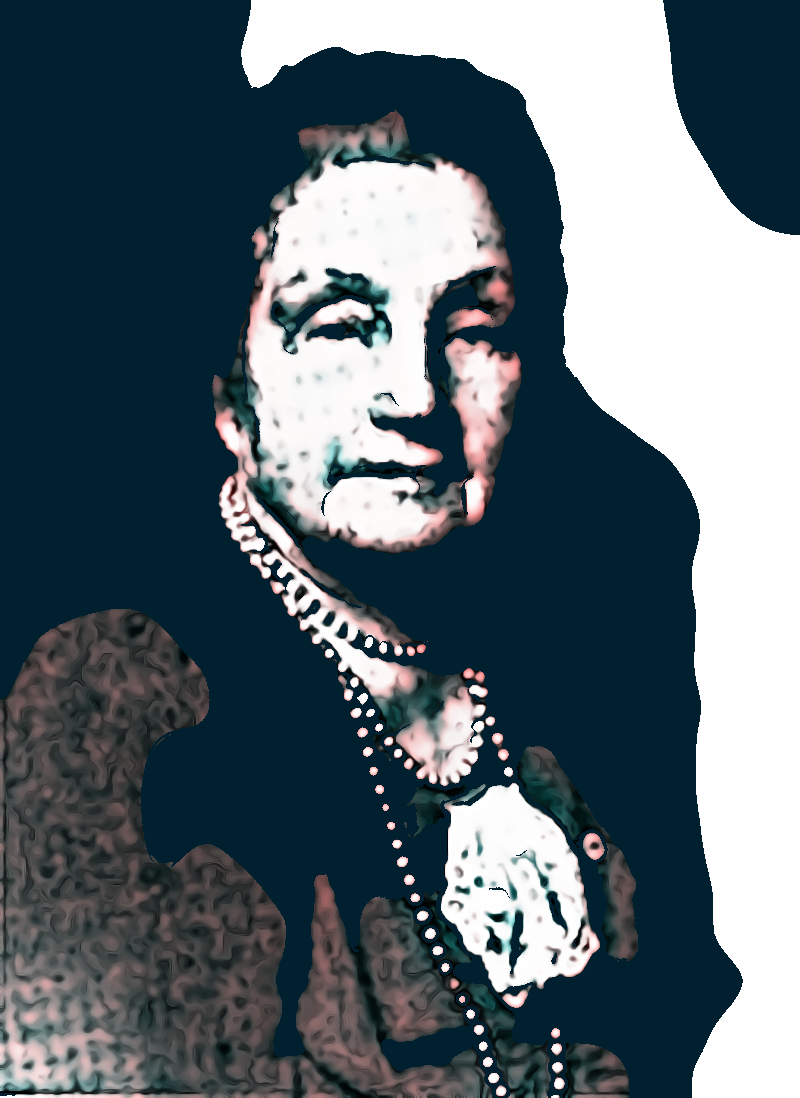
\includegraphics[width=10cm]{winifred_merrill}};
			%
			\draw [fill=galaxy, ultra thick] (3.4,-6.5) rectangle (12.6,-7.5);
			\node at (8,-7) {\textcolor{black}{\fontsize{18}{19}\selectfont Winifred Edgerton Merrill}};
			%
			\draw [fill=title, thick] (14,6.85) rectangle (27,7.75);
			\node (example-textwidth-2) [right, align=left, text width=12cm, color=black, font=\fontsize{18pt}{19pt}\selectfont] at (15,7.35) {\textbf{24 settembre 1862}};
			%
			\node (example-textwidth-2) [right, align=left, text width=12cm, color=black, font=\fontsize{18pt}{19pt}\selectfont] at (15,6) {Matematica e astronoma};
			%
			\draw [fill=dida, thick] (14,5.1) rectangle (27,1.9);
			\node (example-textwidth-2) [right, align=left, text width=10cm, color=black, font=\fontsize{18pt}{19pt}\selectfont] at (15,3.5) {A 16 anni calcola l'orbita della cometa Pons-Brooks a partire dai dati forniti dall'osservatorio di Harvard.};
			%
			\draw [fill=title, thick] (14,1.3) rectangle (27,0.4);
			\node (example-textwidth-2) [right, align=left, text width=12cm, color=black, font=\fontsize{18pt}{19pt}\selectfont] at (15,0.8) {\textbf{4 febbraio 1884}};
			%
			\node (example-textwidth-2) [right, align=left, text width=10cm, color=black, font=\fontsize{18pt}{19pt}\selectfont] at (15,-2.9) {Grazie a \textbf{Frederick Barnard} le viene concesso l'uso del telescopio della \emph{Columbia University} come assistente di \textbf{John Rees}.\\Una delle condizioni, però, era \emph{non disturbare gli studenti maschi}...};
			%
			\shade [bottom color=paper02,top color=paper01] (14,-6) rectangle (27,-14);
			\draw [thick] (14,-6) rectangle (27,-14);
			\node (example-textwidth-2) [right, align=left, text width=11cm, color=black, font=\fontsize{18pt}{19pt}\selectfont] at (15,-10) {In considerazione della straordinaria eccellenza del lavoro scientifico svolto da Miss Winifred Edgerton, come attestato dai professori che la sovrinteso il suo corso in Astronomia pratica e in Matematica Pura, (...) il grado di \emph{Doctor of Philosophy} può essere conferito a Miss Edgerton \emph{cum laude}.};
			%
			\node (example-textwidth-2) [right, align=left, text width=11cm, color=black, font=\fontsize{18pt}{19pt}\selectfont] at (15,-16.5) {Ha scritto un libro di matematica e musica con il genero \textbf{Robert Russell Bennett}, compositore e vincitore dell'Oscar per la colonna sonora del \emph{musical} \emph{Oklahoma!}};
			%
			\draw [fill=title, thick] (14,-19.1) rectangle (27,-20);
			\node (example-textwidth-2) [right, align=left, text width=12cm, color=black, font=\fontsize{18pt}{19pt}\selectfont] at (15,-19.5) {\textbf{6 settembre 1951}};
		\end{scope}
		%
		% Henrietta Swan Leavitt
		%
		\begin{scope}[shift={(0,-46.5)}]
			\foreach \i in {0,1,...,11}
			{
				\draw [fill=white, thick] (14.75+\i,8.8) rectangle (15.25+\i,9.3);
			}
			%
			\draw [thick] (3,6.55) rectangle (13,-6.55);
			\node at (8,0) {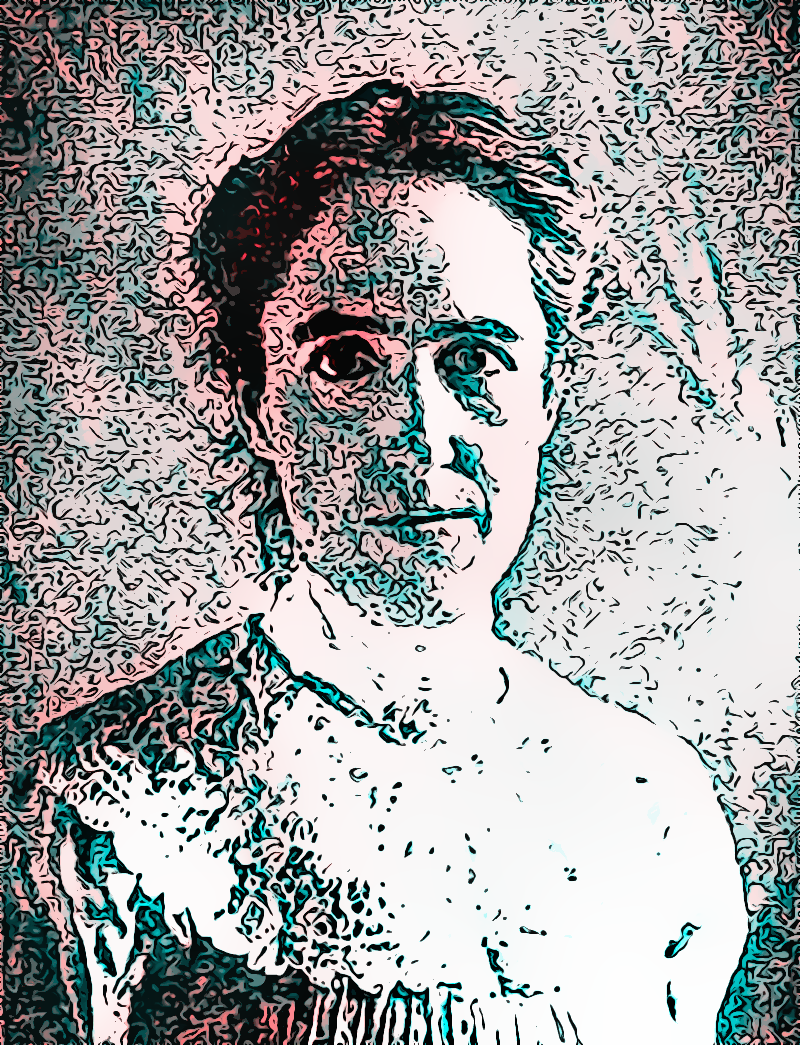
\includegraphics[width=10cm]{henrietta_swan}};
			%
			\draw [fill=galaxy, ultra thick] (3.8,-6.2) rectangle (12.2,-7.2);
			\node at (8,-6.7) {\textcolor{black}{\fontsize{18}{19}\selectfont Henrietta Swan Leavitt}};
			%
			\draw [fill=title, thick] (14,6.55) rectangle (27,7.45);
			\node (example-textwidth-2) [right, align=left, text width=12cm, color=black, font=\fontsize{18pt}{19pt}\selectfont] at (15,6.95) {\textbf{4 luglio 1868}};
			%
			\node (example-textwidth-2) [right, align=left, text width=10cm, color=black, font=\fontsize{18pt}{19pt}\selectfont] at (15,5.6) {Astronoma};
			%
			\draw [fill=space, thick] (14,-2.5) rectangle (27,4.8);
			\node (example-textwidth-2) [right, align=left, text width=10cm, color=white, font=\fontsize{18pt}{19pt}\selectfont] at (15,1.1) {Dopo la laurea, ha iniziato a lavorare presso l'Osservatorio Astronomico di Harvard, il cui direttore, \textbf{Edward Charles Pickering}, pensava che l'obiettivo dell'Osservatorio fosse collezionare più dati possibile sulle stelle in modo da supportare i modelli teorici.};
			%
			\node (example-textwidth-2) [right, align=left, text width=11cm, color=black, font=\fontsize{18pt}{19pt}\selectfont] at (15,-5.8) {Mirava a tabulare posizione, colore e magnitudine di quante più stelle possibile. Felice di avere l'assisteza della Leavitt senza doverla pagare, le diede il compito di studiare le lastre fotograriche dalle quali ricavare i dati da registrare.};			
			% 
			\shade [bottom color=paper02,top color=paper01] (14,-9) rectangle (27,-17);
			\draw [thick] (14,-9) rectangle (27,-17);
			\node (example-textwidth-2) [right, align=left, text width=11cm, color=black, font=\fontsize{18pt}{19pt}\selectfont] at (15,-13) {Nel corso di questo lavoro di raccolta e catalogazione scoprì una nuova classe di stelle, oggi note come \emph{cefeidi}, che presentavano \emph{una notevole relazione tra la luminosità di queste variabili e la durata dei loro periodi}. La scoperta di Henrietta ha permesso di determinare le distanze nell'universo.};			
			%
			\draw [fill=title, thick] (14,-17.8) rectangle (27,-18.7);
			\node (example-textwidth-2) [right, align=left, text width=12cm, color=black, font=\fontsize{18pt}{19pt}\selectfont] at (15,-18.3) {\textbf{12 dicembre 1921}};
			%
			\node (example-textwidth-2) [right, align=left, text width=12cm, color=black, font=\fontsize{18pt}{19pt}\selectfont] at (15,-21.5) {Nel 1925, non sapendo della sua scomparsa, \textbf{Gösta Mittag-Leffler} scrisse una lettera indirizzata a Henrietta Leavitt per comunicarle che sarebbe stata inserita nelle nomine per il Premio Nobel per la fisica del 1926.};
		\end{scope}
		%
		% Cecilia Payne-Gaposchkin
		%
		\begin{scope}[shift={(0,-77.5)}]
			\foreach \i in {0,1,...,11}
			{
				\draw [fill=white, thick] (14.75+\i,6.4) rectangle (15.25+\i,5.9);
			}
			%
			\draw [thick] (3,3.95) rectangle (13,-3.95);
			\node at (8,0) {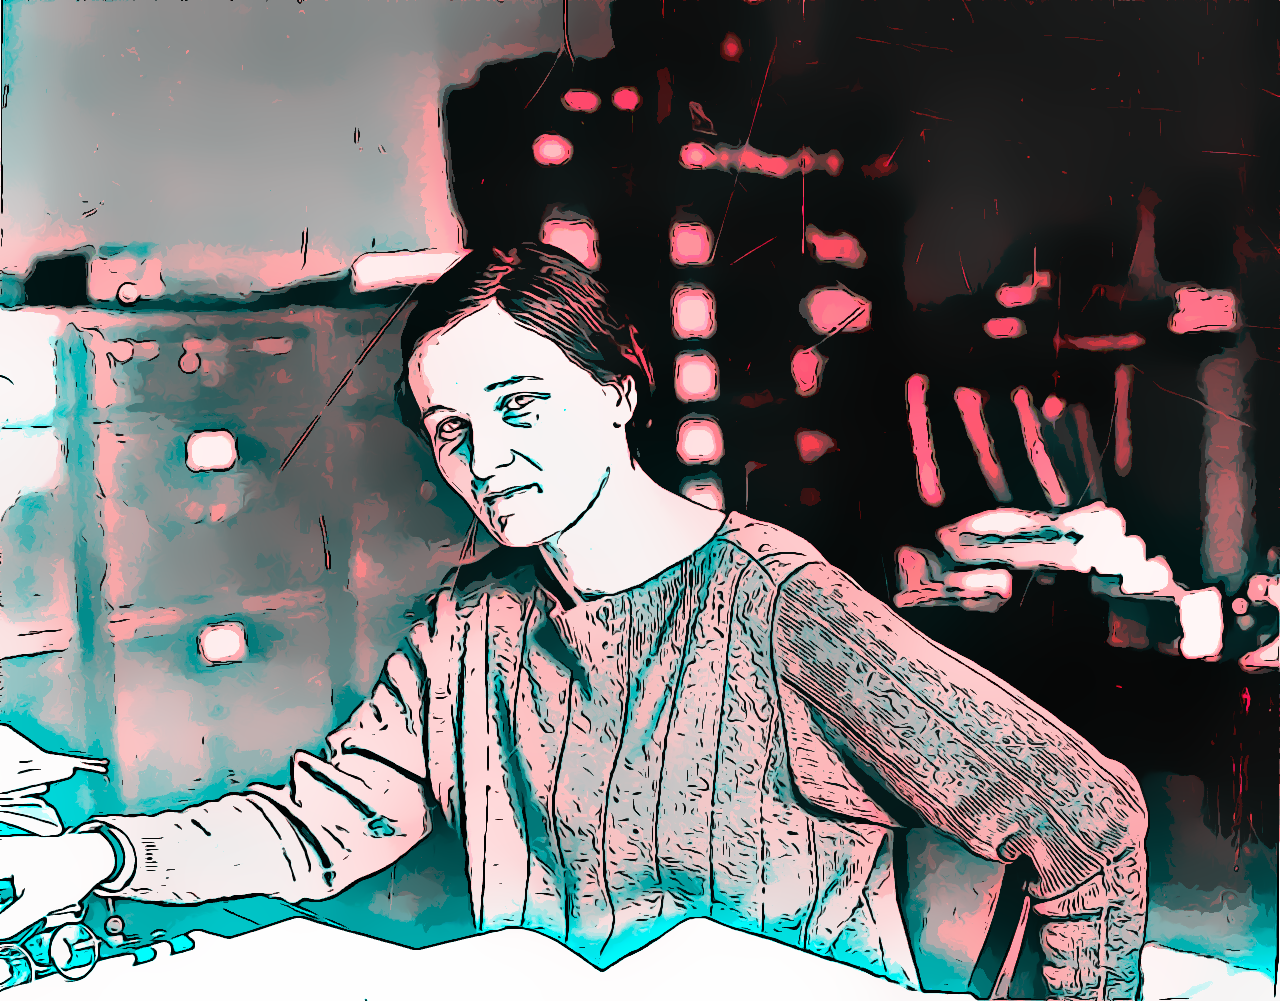
\includegraphics[width=10cm]{cecilia_payne}};
			%
			\draw [fill=galaxy, ultra thick] (3.6,-3.6) rectangle (12.4,-4.6);
			\node at (8,-4.1) {\textcolor{black}{\fontsize{18}{19}\selectfont Cecilia Payne-Gaposchkin}};
			%
			\draw [fill=title, thick] (14,3.95) rectangle (27,4.85);
			\node (example-textwidth-2) [right, align=left, text width=12cm, color=black, font=\fontsize{18pt}{19pt}\selectfont] at (15,4.35) {\textbf{10 maggio 1900}};
			%
			\node (example-textwidth-2) [right, align=left, text width=10cm, color=black, font=\fontsize{18pt}{19pt}\selectfont] at (15,1.8) {Si appassiona all'astronomia dopo aver assistito a una conferenza di \textbf{Arthur Eddington} sulla sua spedizione del 1919.};		
			%
			\draw [fill=dida, thick] (14,-0.2) rectangle (27,-8.2);
			\node (example-textwidth-2) [right, align=left, text width=10cm, color=black, font=\fontsize{18pt}{19pt}\selectfont] at (15,-4.2) {Nel 1922 \textbf{Harlow Shapley}, all'epoca direttore dell'Osservatorio di Harvard, aveva dato inizio a un programma di borse e assegni per incentivare le donne astronome a lavorare presso il suo Osservatorio. Cecilia, alureatasi a Cambridge, si trasferì dall'Inghilterra agli Stati Uniti nel 1923.};
			%
			\node (example-textwidth-2) [right, align=left, text width=12cm, color=black, font=\fontsize{18pt}{19pt}\selectfont] at (15,-10.2) {Nel 1925 ottenne il dottorato con una tesi che \textbf{Otto Struve} definì come \emph{la più brillante tesi di dottorato mai scritta in astronomia}.};
			%
			\shade [bottom color=paper02,top color=paper01] (14,-12.2) rectangle (27,-20.4);
			\draw [thick] (14,-12.2) rectangle (27,-20.4);
			\node (example-textwidth-2) [right, align=left, text width=11cm, color=black, font=\fontsize{18pt}{19pt}\selectfont] at (14.8,-16.2) {\emph{Cecilia Payne, che ha studiato la nuova scienza della fisica quantistica, sapeva che le strutture caratteristiche nello spettro di ciascun atomo erano determinare dalla configurazione degli elettroni. Ella sapeva anche che alle alte temperature, uno o più elettroni vengono strappati agli atomi, che così diventano ioni.}};
			%
			\draw [fill=title, thick] (14,-21.2) rectangle (27,-22.1);
			\node (example-textwidth-2) [right, align=left, text width=12cm, color=black, font=\fontsize{18pt}{19pt}\selectfont] at (15,-21.7) {\textbf{7 dicembre 1979}};
		\end{scope}
		% image credits
		\begin{scope}[shift={(0,-103)}]
			\draw [fill=space,thick] (2,1) rectangle (28,-1);
			%
			\node (example-textwidth-2) [right, align=left, text width=25cm, color=white, font=\fontsize{18pt}{19pt}\selectfont] at (2.5,0) {Le immagini sono tratte dalle rispettive voci su Wikipedia e poi rielaborate graficamente usando il filtro G'MIC-Qt di Gimp.};
		\end{scope}
		%
		\begin{scope}[shift={(0,-105)}]
			\node at (27,0) () {
\includegraphics[width=3.7cm]{licenza}};
			\node (example-textwidth-2) [right, align=left, text width=14cm, color=black, font=\fontsize{14pt}{15pt}\selectfont] at (12.5,-0.1) {Testo e grafica: @ulaulaman - Gianluigi Filippelli};
		\end{scope}
	\end{tikzpicture}
\end{document}
